\documentclass{article}
\usepackage{graphicx} % Required for inserting images
\usepackage[margin=1in]{geometry}
\usepackage{amsmath}
\usepackage{hyperref}
\usepackage{xcolor}
\usepackage{listings}
\usepackage{xparse}
\usepackage{booktabs}
\NewDocumentCommand{\codeword}{v}{%
\texttt{\textcolor{blue}{#1}}%
}

\title{CX 4230 - Computer Simulation - Project 3}
\author{Reetesh Sudhakar \& Roshan Desai}
\date{April 26th, 2024}

\begin{document}

\maketitle

\section{Task 1: Create a simulator}
In order to verify the simulation code, we went through a few main steps that really tested the implementation and made sure the outputs were correct. First, we ensured that we were capturing all the right behaviors, such as rider arrivals, station selection, bike availability, ride durations, and return destinations. \\ \\
Once we had verified that our simulation took all those into account, we then had to make sure we were considering all the correct parameters, such as the number of riders ({\tt n}), distribution for bike use time {\tt mu} and {\tt sigma}, and riders per minute ({\tt \_lambda}). Finally, once we knew we were simulating the right thing, we ran some sanity checks with simple cases. Through running the simulation on a very simple 10 bikes per station, we found out that our initial simulation had a success rate that was a lot higher than expected! We also noted that the wait times were not being used correctly - we were simply logging the arrival time and not adding individuals waiting for a bike back into the simulation. \\ \\ 
Realizing this, we decided to refactor our code into the {\tt BikeshareSimulation} class, which can be found in the Jupyter Notebook. We opted for an event driven approach, wherein we create arrival and return events and continually sort and process them. This allowed us to account for wait times for individuals properly. We also used this new opportunity to fix another bug, where we weren't accounting for the right terminating conditions for the simulation. We initially were calculating the success rate based off of the hardcoded number of individuals for Task 2 ($n = 3500$), but did not account for the fact that the 24 hours could occur before all 3500 individuals arrive. We then realized we had to also track the number of riders arriving within the 24-hour period and use that for our success rate calculation instead. \\ \\ 
Once we had written this updated simulation, we validated our output by seeding the data and making sure that our simulation matched up exactly with a sample simulation we had created. By doing these tests, we were able to ensure our simulation works as expected and even catch a flaw that we had missed in our initial implementation.

\section{Task 2: A baseline experiment}
Using the parameters specified ({\tt n=3500, $\lambda$=2.38, $\mu$=2.78, and $\sigma$=0.619}, and the probability values specified in the csv files, we yielded a 90\% confidence interval $$(0.8700801254620589, 0.8882055888236553)$$ Other descriptive statistics we recorded for this simulation were as follows: \\\\
\begin{tabular}{rr}
    probability of successful rental & 0.8791 \\
    average waiting time (for riders who got a bike) & 20.4681 minutes \\
    average ride time (for riders who got a bike) & 19.0629 minutes
\end{tabular} \\\\
Details for the baseline experiment can be found in the Jupyter Notebook. 

\newpage
\section{Task 3: An "idealized" experiment}
\begin{tabular}{rrrr}
\toprule
Number of bikes per station & Probability of a successful rental & Average waiting time & Average ride time \\
\midrule
1 & 0.071957 & 30.481331 & 18.414169 \\
2 & 0.159622 & 35.705521 & 18.642338 \\
3 & 0.256000 & 35.982701 & 18.395302 \\
4 & 0.347146 & 37.191874 & 19.148582 \\
5 & 0.486838 & 39.427267 & 19.650106 \\
6 & 0.595245 & 42.019717 & 19.717366 \\
7 & 0.666667 & 39.209755 & 19.425271 \\
8 & 0.726699 & 36.002540 & 19.804278 \\
9 & 0.876286 & 19.802257 & 19.421940 \\
10 & 0.835143 & 26.168508 & 19.692057 \\
11 & 0.965629 & 9.763847 & 19.455909 \\
12 & 0.942286 & 10.860133 & 19.830028 \\
13 & 0.969644 & 3.987259 & 19.791042 \\
14 & 0.970740 & 7.047446 & 19.877152 \\
15 & 0.986000 & 2.260351 & 19.480216 \\
16 & 0.999135 & 1.615585 & 19.840298 \\
17 & 0.989714 & 2.027131 & 19.274397 \\
18 & 1.000000 & 0.082064 & 19.441390 \\
19 & 0.990610 & 2.007152 & 19.818418 \\
20 & 1.000000 & 0.000042 & 19.370865 \\
21 & 0.997928 & 0.581875 & 19.119011 \\
22 & 1.000000 & 0.000000 & 19.431787 \\
23 & 0.999134 & 0.122368 & 19.328673 \\
24 & 0.998257 & 0.339932 & 19.685136 \\
25 & 1.000000 & 0.000000 & 19.505083 \\
26 & 0.993429 & 0.513703 & 19.139258 \\
27 & 1.000000 & 0.000000 & 19.719982 \\
28 & 0.998000 & 0.068838 & 19.165527 \\
29 & 1.000000 & 0.000000 & 19.385431 \\
30 & 0.997279 & 0.173117 & 19.755661 \\
31 & 0.998256 & 0.527393 & 19.669985 \\
32 & 1.000000 & 0.000000 & 19.586807 \\
33 & 1.000000 & 0.000000 & 19.101658 \\
34 & 1.000000 & 0.000000 & 19.381338 \\
35 & 1.000000 & 0.000000 & 19.607769 \\
36 & 1.000000 & 0.000000 & 19.825058 \\
37 & 1.000000 & 0.000000 & 19.434306 \\
38 & 1.000000 & 0.000000 & 19.492338 \\
39 & 1.000000 & 0.000000 & 19.457210 \\
40 & 1.000000 & 0.000000 & 19.876705 \\
41 & 1.000000 & 0.000000 & 19.441862 \\
42 & 1.000000 & 0.000000 & 19.629161 \\
43 & 1.000000 & 0.000000 & 19.171897 \\
44 & 1.000000 & 0.000000 & 19.461251 \\
45 & 1.000000 & 0.000000 & 19.429790 \\
46 & 1.000000 & 0.000000 & 19.619667 \\
47 & 1.000000 & 0.000000 & 19.095062 \\
48 & 1.000000 & 0.000000 & 19.559105 \\
49 & 1.000000 & 0.000000 & 19.441488 \\
50 & 1.000000 & 0.000000 & 19.777372 \\
\bottomrule
\end{tabular}

\begin{figure}[!h]
    \centering
    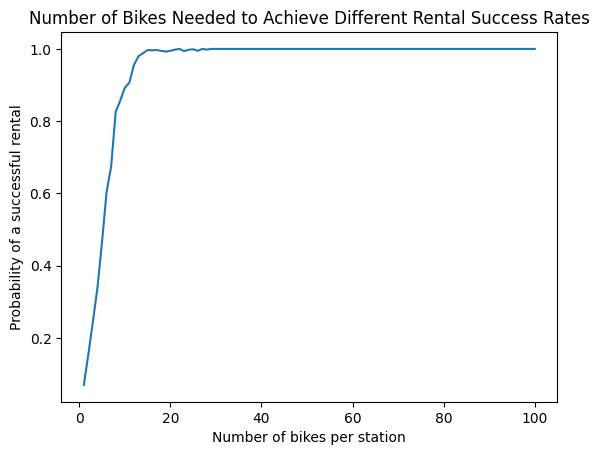
\includegraphics[width=0.9\linewidth]{assets/3.png}
\end{figure}
We ran our simulation for a number of bikes per station from 0-100. The table above shows the results of the first 50, because after that the results stabilized for the most part and the variance in average ride time was only due to randomness. As shown in the above table and figure, after about 30 bikes per station, the success rate of a rental stabilized at 100\%, so this is minimum number of bikes that could be made available to meet demand fully.

\newpage
\section{Task 4: Checking assumptions}
\begin{figure}[!h]
    \centering
    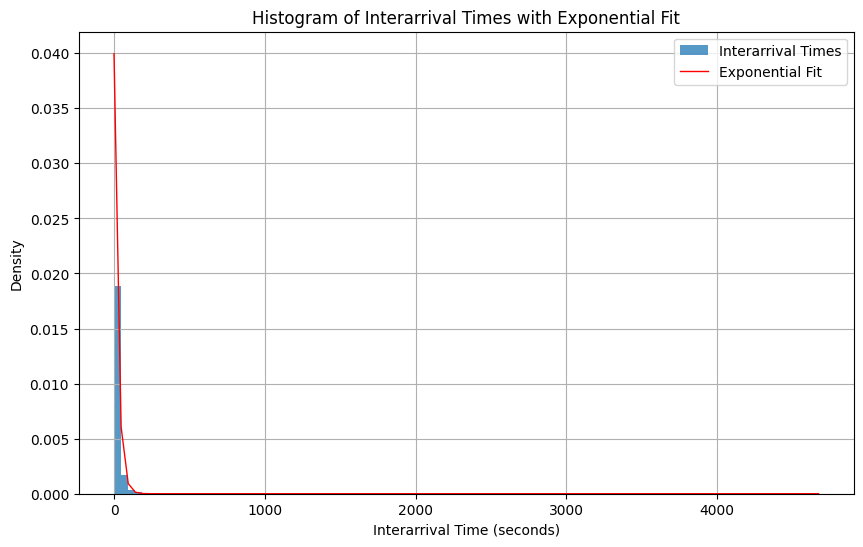
\includegraphics[width=0.9\linewidth]{assets/4.png}
\end{figure}

\subsection{Analysis of Interarrival Times}
After truncating the data to the specified time range, we computed some  descriptive statistics: \\\\
\begin{tabular}{rr}
    count & 207117.000000 \\
    mean & 25.028689 \\
    std & 67.762992 \\
    min & 0.000000 \\
    25\% & 5.000000 \\ 
    50\% & 12.000000 \\
    75\% & 26.000000 \\
    max & 4673.000000 \\
\end{tabular} \\\\
\textbf{Re:} Exponential Distribution: The fit suggests some adherence to an exponential model, especially for smaller interarrival times, but the distribution has a long tail, which is not typical for a pure exponential distribution. This indicates the presence of \textbf{very} long interarrival times relative to the mean. \\\\
\textbf{Re:} Stationarity and Independence: The wide range and the high standard deviation compared to the mean might suggest that the interarrival times are influenced by factors that change over time (e.g., rush hours, weekends vs weekdays, and also just popular locations themselves), which challenges the assumption of stationarity and independence typically required for a process to be well-modeled. \\\\
\textbf{Concluding thoughts:} While there's a resemblance to an exponential distribution for shorter intervals (which makes sense - lots of people usually just rent these bikes to quickly get from point A to point B), the presence of very long interarrival times and the large standard deviation suggest that the process might not be entirely stationary or independent. Factors such as time of day, day of the week, tourism, and many other things, could significantly affect the interarrival times shown in the dataset.

\end{document}
